\documentclass{exam}
\usepackage{../commonheader}
\lstset{language=Scheme}

%%% CHANGE THESE %%%%%%%%%%%%%%%%%%%%%%%%%%%%%%%%%%%%%%%%%%%%%%%%%%%%%%%%%%%%%%
\discnumber{10}
\title{\textsc{SQL and Final Review}}
\date{November 27 to December 1, 2017}
%%%%%%%%%%%%%%%%%%%%%%%%%%%%%%%%%%%%%%%%%%%%%%%%%%%%%%%%%%%%%%%%%%%%%%%%%%%%%%%

\begin{document}
\maketitle
\rule{\textwidth}{0.15em}
\fontsize{12}{15}\selectfont

\section{Creating Tables, Querying Data}
Examine the table, \texttt{mentors}, depicted below.
\begin{center}
\begin{tabular}{ |c|c|c|c|c| }
 \hline
 \textbf{Name} & \textbf{Food} & \textbf{Color} & \textbf{Editor} & \textbf{Language} \\
 \hline
 Tiffany & Thai & Purple & Notepad++ & Java \\
 \hline
 Diana & Pie & Green & Sublime & Java \\
 \hline
  Allan & Sushi & Orange & Emacs & Ruby \\
 \hline
 Alfonso & Tacos & Blue & Vim & Python \\
 \hline
 Kelly & Ramen & Green & Vim & Python \\
 \hline
\end{tabular}
\end{center}
\begin{questions}
\question Create a new table \textbf{mentors} that contains all the information above.
(You only have to write out the first two rows.)
\begin{solution}
\begin{lstlisting}[language=SQL]
create table mentors as
    select 'Tiffany' as name, 'Thai' as food, 'Purple' as color, 'Notepad++' as editor, 'Java' as language union
    select 'Diana', 'Pie', 'Green', 'Sublime', 'Java' union
    select 'Allan', 'Sushi', 'Orange', 'Emacs', 'Ruby' union
    select 'Alfonso', 'Tacos', 'Blue', 'Vim', 'Python' union
    select 'Kelly', 'Ramen', 'Green', 'Vim', 'Python';
\end{lstlisting}
\end{solution}

\clearpage

%%% Question %%%
\begin{blocksection}
\question Write a query that lists all the mentors along with their favorite food if their favorite color is green.\newline
Output:
\begin{lstlisting}
Diana|Pie
Kelly|Ramen
\end{lstlisting}
\begin{solution}[1in]
\begin{lstlisting}[language=SQL]
select m.name, m.food
  from mentors as m
  where m.color = 'Green';

Without aliasing:

select name, food
  from mentors
  where color = 'Green';
\end{lstlisting}
\end{solution}

\question Write a query that lists the food and the color of every person whose
favorite language is NOT Python. \newline
Output:
\begin{lstlisting}
Sushi|Orange
Pie|Green
Thai|Purple
\end{lstlisting}
\begin{solution}[1in]
\begin{lstlisting}[language=SQL]
select m.food, m.color
  from mentors as m
  where m.language <> 'Python';

Without aliasing:

select food, color
  from mentors
  where language != 'Python';
\end{lstlisting}
\end{solution}
\end{blocksection}

%%% Question %%%
\begin{blocksection}
\question Write a query that lists all the pairs of mentors who like the same language. (How can we make sure to remove duplicates?) \newline
Output:
\begin{lstlisting}
Kelly|Alfonso
Tiffany|Diana
\end{lstlisting}
\begin{solution}[2in]
\begin{lstlisting}[language=SQL]
select m1.name, m2.name
    from mentors as m1, mentors as m2
    where m1.language = m2.language and m1.name > m2.name;
\end{lstlisting}
\end{solution}
\end{blocksection}


%%% Question %%%
\begin{blocksection}
\section{Fish Population}
The 61A mentors want to start a fish hatchery, and they need your help to analyze the data they've collected for the fish populations! Also, running a hatchery is expensive -- they'd like to make some money on the side by selling some seafood (only older fish of course) to make delicious sushi. \newline
\newline
The following table contains a subset of the data that has been collected. The SQL column names are listed in brackets. Note: we must be able to extend your queries to larger tables! (i.e, don't hard code your answers) \newline
\newline
Table name: \texttt{fish}*
\begin{center}
\begin{tabular}{ |c|c|c|c|c| }
 \hline
 \textbf{Species} & \textbf{Population} & \textbf{Breeding Rate} & \textbf{\$/piece} & \textbf{\# of pieces per fish} \\
  \textbf{[species]} & \textbf{[pop]} & \textbf{[rate]} & \textbf{[price]} & \textbf{[pieces]} \\
 \hline
 Salmon & 500 & 3.3 & 4 & 30 \\
 \hline
 Eel & 100 & 1.3 & 4 & 15 \\
 \hline
  Yellowtail & 700 & 2.0 & 3 & 30 \\
 \hline
 Tuna & 600 & 1.1 & 3 & 20 \\
 \hline
\end{tabular}
\end{center}
*(This was made with fake data, do not actually sell fish at these rates)
\question \textbf{Aggregation} Hint: The aggregate functions \texttt{MAX}, \texttt{MIN}, \texttt{COUNT}, and \texttt{SUM} return the maximum, minimum, number, and sum of the values in a column. The  \texttt{GROUP BY} clause of a select statement is used to partition rows into groups.

\begin{parts}

\part Write a query to find the three most populated fish species.
\begin{solution}[0.5in]
\begin{lstlisting}[language=SQL]
select species from fish order by -pop LIMIT 3;
\end{lstlisting}
\end{solution}

\part Profit is good, but more profit is better. Write a query to select the species that yields the most number of pieces for each price. Your output should include the species, price, and pieces.
\begin{solution}[0.5in]
\begin{lstlisting}[language=SQL]
select species, price, MAX(pieces) from fish GROUP BY price;
\end{lstlisting}
\end{solution}

\end{parts}

\end{blocksection}

\begin{blocksection}
\vspace{10px}
(c) Write a query to find the total number of fish in the "ocean." Additionally, include the number of species we summed. Your output should have the number of species and the total population.
\begin{solution}[0.5in]
\begin{lstlisting}[language=SQL]
select COUNT(species), SUM(pop) from fish;
\end{lstlisting}
\end{solution}

\end{blocksection}

\begin{blocksection}
\vspace{10px}
(d) Business is good, but a bunch of competition has sprung up! Through some cunning corporate espionage, we have determined that one such competitor plans to open shop with the following rates:\newline
\newline
Table name: \texttt{competitor}
\begin{center}
\begin{tabular}{ |c|c| }
 \hline
 \textbf{Species} & \textbf{\$/piece} \\
  \textbf{[species]} & \textbf{[price]} \\
 \hline
 Salmon & 2 \\
 \hline
 Eel & 3.4 \\
 \hline
  Yellowtail & 3.2  \\
 \hline
 Tuna & 2.6  \\
 \hline
\end{tabular}
\end{center}
Write a query that returns, for each species, the difference between our hatchery’s revenue versus the competitor’s revenue for one whole fish. For example, the table should contain the following row: \newline
\texttt{Salmon | 60} \newline \newline
We make 30 pieces of salmon at \$4 for a total revenue of \$120, whereas the competitor makes 30 pieces at \$2 a piece for a total revenue of \$60. The difference is \$60. Remember to do this for every species!
\begin{solution}[1in]
\begin{lstlisting}[language=SQL]
select fish.species, (fish.price - competitor.price) * pieces
    from fish, competitor
    where fish.species = competitor.species;
\end{lstlisting}
\end{solution}


\end{blocksection}

\question \textbf{Recursive Select} Suppose these fish breed every day. The population of each fish gets multiplied by its breeding rate every year. Write a recursive select query that creates a table of fish 10 years from now.

\begin{solution}[0.5in]
\begin{lstlisting}[language=SQL]
with
  annual_pop(yearly_species, yearly_pop, N) as (
     select species, pop, 0 from fish union
     select yearly_species, yearly_pop * rate, N + 1
         from annual_pop, fish
         where yearly_species = species and N < 10
  )
select yearly_species, yearly_pop from annual_pop where N = 10;

\end{lstlisting}
\end{solution}


\end{questions}

\pagebreak


{\huge \vspace*{0.5cm} \textsc{Final Review}}


\rule{\textwidth}{0.15em}

\section{Environment Diagrams}
\begin{questions}

\begin{blocksection}
\question Draw the environment diagram for the following code snippet:
\begin{lstlisting}
def one(two):
    three = two
    def four(five):
        nonlocal three
        if len(three) < 1:
            three.append(five)
            five = lambda x: four(x)
        else:
            five = seven + 7
        return five
    two = two + [1]
    seven = 8
    return four(three)

eight = one([])
print(eight(9))
\end{lstlisting}
\end{blocksection}

\begin{solution}
\url{https://goo.gl/d71WTd}
\linebreak
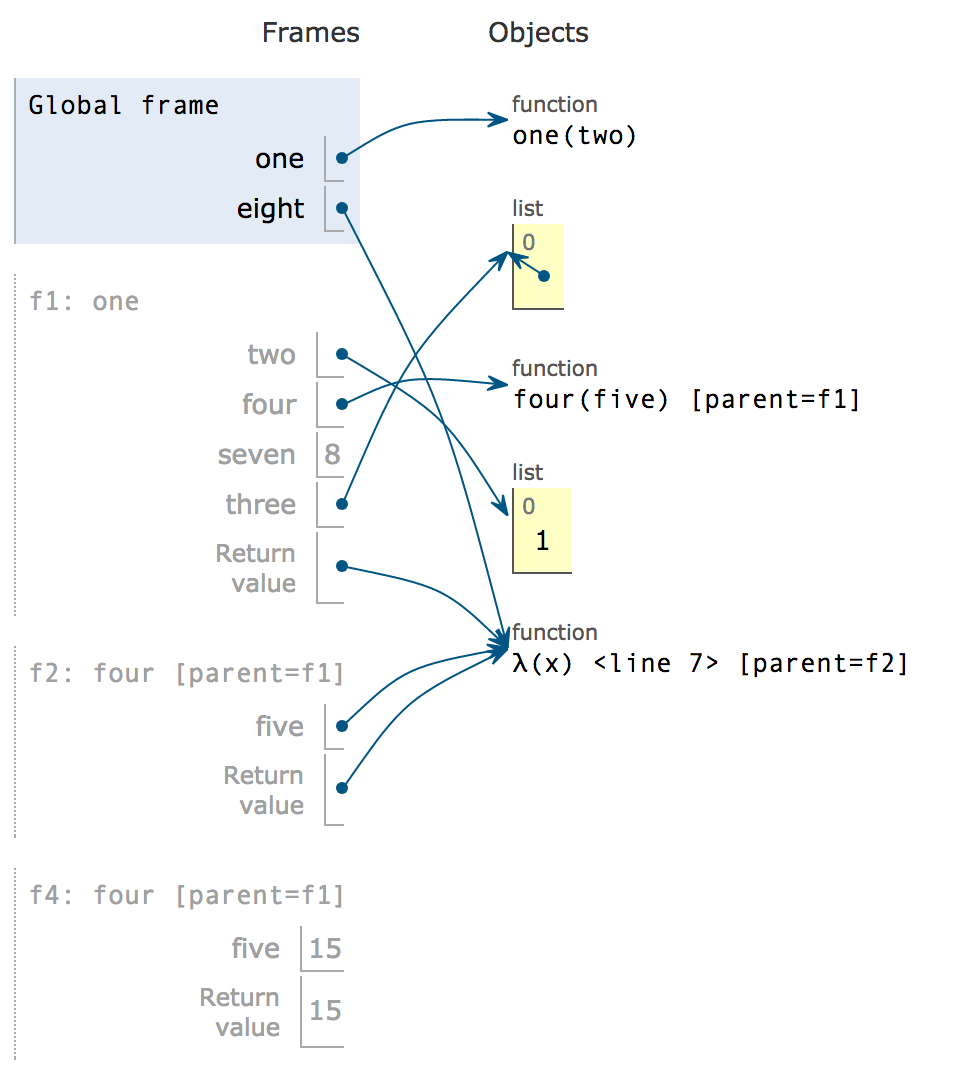
\includegraphics[width=0.85\textwidth]{envdiag}

\end{solution}

\section{Recursive Data Structures}

\begin{blocksection}
\question DoubleTree hired you to architect one of their hotel expansions!  As
you might expect, their floor plan can be modeled as a tree and the expansion
plan requires doubling each node (the patented double tree floor plan). Here's
what some sample expansions look like:\\\\
\begin{tabular}{c c}
\textbf{Before} & \textbf{After}\\
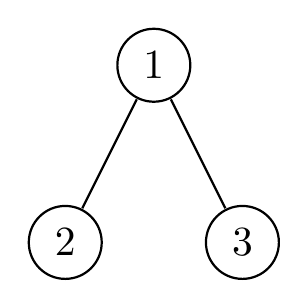
\begin{tikzpicture}[thick, scale=1.5, transform shape]
    \node [circle, draw] (z){$1$}
        child {node [circle, draw] (a) {$2$}}
        child {node [circle, draw] (b) {$3$}}
        ;
\end{tikzpicture}
&
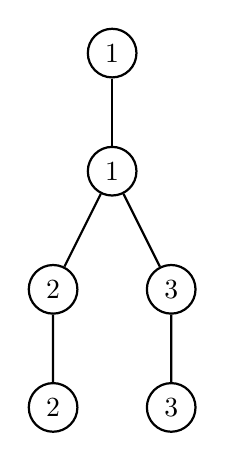
\begin{tikzpicture}[thick, scale=1.0, transform shape]
    \node [circle, draw] (z){$1$}
        child {node [circle, draw] (a) {$1$}
            child {node [circle, draw] (b) {$2$}
                child {node [circle, draw] (d) {$2$}}
            }
            child {node [circle, draw] (c) {$3$}
                child {node [circle, draw] (e) {$3$}}
            }
        }
        ;
\end{tikzpicture}
\end{tabular}

Fill in the implementation for \texttt{double\char`_tree}.

\begin{lstlisting}
def double_tree(t):
    """
    Given a tree, return a new tree where entries appear
    twice.
    >>> double_tree(Tree(1))
    Tree(1, [Tree(1)])
    >>> double_tree(Tree(1, [Tree(2), Tree(3)]))
    Tree(1, [Tree(1, [Tree(2, [Tree(2)]),
                      Tree(3, [Tree(3)])
                     ])
            ])
    """
\end{lstlisting}
\begin{solution}[0.5in]
\begin{lstlisting}
    if t.is_leaf():
        return Tree(t.label, [Tree(t.label)])
    else:
        dbl_branches = [double_tree(c) for c in t.branches]
            return Tree(t.label,
                        [Tree(t.label, dbl_branches)])
\end{lstlisting}
\end{solution}
\end{blocksection}

\begin{blocksection}
\question Fill in the implementation of \texttt{double\char`_link}.

\begin{lstlisting}
def double_link(lst):
    """
    Using mutation, replaces the second in each pair of items
    with the first. The first of each pair stays as is. Returns the list.
    >>> double_link(Link(1, Link(2, Link(3, Link(4)))))
    Link(1, Link(1, Link(3, Link(3))))
    >>> double_link(
            Link('c', Link('s', Link(6, Link(1, Link('a')))))
        )
    Link('c', Link('c', Link(6, Link(6, Link('a')))))
    """
    if __________________________________________:
        return __________________________________
    _____________________________________________
    _____________________________________________
    return ______________________________________
\end{lstlisting}
\begin{solution}[0.5in]
\begin{lstlisting}
    if lst is Link.empty or lst.rest is Link.empty:
        return lst
    lst.rest.first = lst.first
    double_link(lst.rest.rest)
    return lst
\end{lstlisting}
\end{solution}
\end{blocksection}

\begin{blocksection}
\question Fill in the implementation of \texttt{shuffle}.

\begin{lstlisting}
def shuffle(lst):
    """
    Swaps each pair of items in a linked list.
    >>> shuffle(Link(1, Link(2, Link(3, Link(4)))))
    Link(2, Link(1, Link(4, Link(3))))
    >>> shuffle(
            Link('s', Link('c', Link(1, Link(6, Link('a')))))
        )
    Link('c', Link('s', Link(6, Link(1, Link('a')))))
    """
    if _________________________________________________
        return _______________________________________
    new_head = lst.rest
    lst.rest = _________________________________________
    ____________________________________________________
    return _____________________________________________
\end{lstlisting}

\begin{solution}[0.5in]
\begin{lstlisting}
    if lst == Link.empty or lst.rest == Link.empty:
        return lst
    new_head = lst.rest
    lst.rest = shuffle(new_head.rest)
    new_head.rest = lst
    return new_head
\end{lstlisting}
\end{solution}
\end{blocksection}

\section{Scheme}

\begin{blocksection}
\question Write a Scheme function \texttt{insert} that creates a new list that would
result from inserting an item into an existing list at the given index. Assume
that the given index is between 0 and the length of the original list,
inclusive.

\begin{lstlisting}[language=Scheme]
(define (insert lst item index)



)
\end{lstlisting}

\begin{solution}
\begin{lstlisting}[language=Scheme]
(define (insert lst item index)
  (if (= index 0)
    (cons item lst)
    (cons (car lst) (insert (cdr lst) item (- index 1))))
)
\end{lstlisting}
\end{solution}

\textbf{Extra:} Write this as a tail recursive function. Assume append is tail
recursive.
\begin{solution}
\begin{lstlisting}[language=Scheme]
(define (insert lst item index)
  (define (helper lst index so-far)
    (if (or (null? lst) (= index 0))
      (append so-far (cons item lst))
      (helper (cdr lst) (- index 1)
              (append so-far (list (car lst))))
    )
  )
  (helper lst index nil)
)
\end{lstlisting}
\end{solution}
\end{blocksection}

\section{Recursive Select in SQL}
\begin{blocksection}
\question Create a \texttt{mod\char`_seven} table that has two columns, a number
from 0 to 100 and then its value mod 7.\\
\textbf{Hint:} You can create a table first with all of the initial data you
will build from, and then build the \texttt{mod\char`_seven} table.

\begin{solution}[1in]
\begin{lstlisting}[language=SQL]
with
    base(n) as (
        select 0 union
        select n+1 from base where n+1<7
    ),
    mod_seven (n, value) as (
        select n, n from base union
        select n+7, value from mod_seven where n+7<=100
    )
select * from mod_seven;

ALTERNATIVE SOLUTION WITH MODULO OPERATOR
with
    mod_seven (n, value) as (
        select 0, 0 union
        select n+1, (n+1)%7 from mod_seven where n<100
     )
select * from mod_seven;

ALTERNATIVE SOLUTION WITH ONE TABLE
(This could be a pre-step to approaching the original solution.)
with
    mod_seven (n, value) as (
        select 0, 0 union
        select 1, 1 union
        select 2, 2 union
        select 3, 3 union
        select 4, 4 union
        select 5, 5 union
        select 6, 6 union
        select n+7, value from mod_seven where n+7 <= 100
    )
select * from mod_seven;
\end{lstlisting}
\end{solution}
\end{blocksection}

\section{Iterators, Generators, and Streams}
\begin{blocksection}
\subimport{../../topics/generators/easy/}{run-length-decoder.tex}

\end{blocksection}

\begin{blocksection}
\subimport{../../topics/streams/scheme/medium/}{puns.tex}

\end{blocksection}

\end{questions}




%%%%%%%%%%%%%%%%%%%%%%%%%%%%%%%%%%%%%%%%%%%%%%%%%%%%%%%%%%%%%%%%%%%%%%%%%%%%%%%

\end{document}